\documentclass[12pt]{article}
\usepackage{graphicx}
\usepackage[utf8]{inputenc}
\usepackage[a4paper, total={6.5in, 9.5in}]{geometry}
\usepackage{float}
\usepackage{hyperref}
\usepackage{titling}
\usepackage{enumitem}
\usepackage{float}
\usepackage{amsmath}
\usepackage{listings}
\usepackage{amssymb}
\usepackage{tikz}
\title{Algorithms: Design \& Analysis - Project Proposal\\\textbf{Hamiltonian Cycle Problem}}
\author{\textbf{Team: Project Team 7}\\Hamad Abdul Razzaq - hr06899 \\Syed Mujtaba Hasan - ms06948 \\Muhammad Meesum Ali Qazalbash - mq06861\\Muhammad . - mm06369}
\date{}

\begin{document}
\maketitle

\section*{Problem Description}
The Hamiltonian Cycle Problem is to find an Hamiltonian Cycle in any given graph. A Hamiltonian Cycle is formally defined as follows:\\
Given an undirected graph $G = \left(V, E\right)$, a Hamiltonian Cycle is a cycle that visits every vertex $V$ exactly once and returns to its starting vertex. So in our Hamiltonian Cycle Problem, we output a sequence of vertices $\langle v_1, v_2, v_3, \ldots, v_n, v_1 \rangle$ where $v_i \in V$ and $(v_i, v_{i+1}) \in E$ and also $(v_1, v_n) \in E$. For example, consider the following graph: \\
\begin{center}
    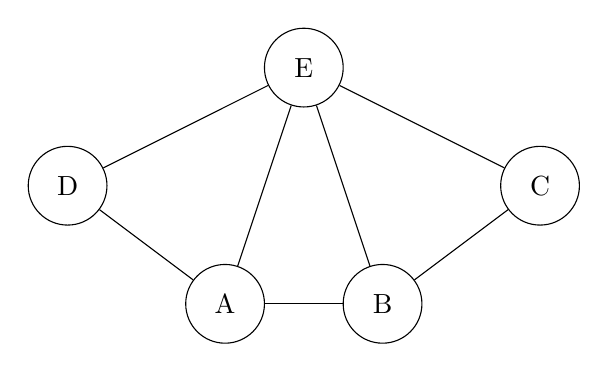
\begin{tikzpicture}
        \node[circle,draw,minimum size=1cm] (A) at (2,0) {A};
        \node[circle,draw,minimum size=1cm] (B) at (4,0) {B};
        \node[circle,draw,minimum size=1cm] (C) at (6,1.5) {C};
        \node[circle,draw,minimum size=1cm] (D) at (0,1.5) {D};
        \node[circle,draw,minimum size=1cm] (E) at (3,3) {E};
        \draw (A) -- (B);
        \draw (C) -- (B);
        \draw (D) -- (A);
        \draw (D) -- (E);
        \draw (C) -- (E);
        \draw (E) -- (B);
        \draw (A) -- (E);
    \end{tikzpicture}
\end{center}
In this graph, the sequence $\langle D, A, B, C, E, D\rangle$ is a Hamiltonian Cycle of the Given graph. This Hamiltonian Cycle is also colored in red below:
\begin{center}
    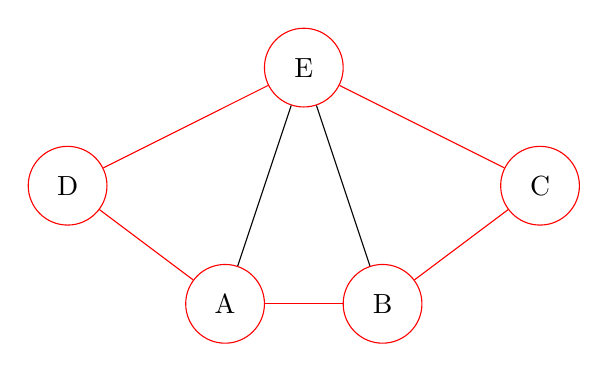
\begin{tikzpicture}
        \node[circle,draw = red,minimum size=1cm] (A) at (2,0) {A};
        \node[circle,draw = red,minimum size=1cm] (B) at (4,0) {B};
        \node[circle,draw = red,minimum size=1cm, ] (C) at (6,1.5) {C};
        \node[circle,draw = red,minimum size=1cm] (D) at (0,1.5) {D};
        \node[circle,draw = red,minimum size=1cm] (E) at (3,3) {E};
        \draw[color=red] (A) -- (B);
        \draw[color=red] (C) -- (B);
        \draw[color=red] (D) -- (A);
        \draw[color=red] (D) -- (E);
        \draw[color=red] (C) -- (E);
        \draw (E) -- (B);
        \draw (A) -- (E);
    \end{tikzpicture}
\end{center}
This is a very famous problem in the graph theory and is characterized as \textbf{NP} complete. This means that for larger graphs, this problem becomes exponentially hard to solve. Although there are many algorithms developed to found the Hamiltonian cycle in the given graph, yet all these algorithms are not efficient one way or the another. To characterize this problem as NP complete is to say that if this problem is solved, then all the other NP problems would also be solvable.

The Hamiltonian Cycle problem has practical significance too. This problem has many real-world applications such as Network routing, scheduling, etc. One benefit that can be inherently seen from the Hamiltonian cycle is that it provides the shortest possible path such that all the nodes in the graph are visited. So in networking, if we have to send a message to every user in the network efficiently, finding Hamiltonian would be of great help here. Moreover, in Robotics \& Autonomous Vehicles, finding Hamiltonian Cycle is helpful in path planning where the Robot or AV has to visit multiple locations and come back at its initial place. This can again be done efficiently by knowing the Hamiltonian Cycle.
\section*{Algorithms / Design Techniques to be explored}
For the above stated problem, we plan to explore the following Algorithms / Design Techniques:
\begin{enumerate}
    \item \textbf{Brute Force Algorithm}
    \item \textbf{Back-tracking Algorithm}
    \item \textbf{Dynamic Programming}
    \item \textbf{Heuristic Algorithms}
\end{enumerate}
The above techniques / algorithms are the ones that we are going to explore at least. We may also end up exploring any other algorithm later on if we find it interesting.
\section*{References}
\begin{enumerate}
    \item \href{https://chat.openai.com/chat}{ChatGPT}. The following prompts were used:
          \begin{itemize}
              \item Formally define Hamiltonian Cycle Problem
              \item Hamiltonian Cycle applications
              \item Algorithms for hamiltonian Cycle problem
          \end{itemize}
    \item \href{https://www.geeksforgeeks.org/hamiltonian-cycle/}{Hamiltonian Cycle - GeeksforGeeks}
\end{enumerate}

\end{document}
